% === A04 - Punteros Vectores y Matrices ===
% David Alejandro Gonzalez Marquez
% dmarquez@dc.uba.ar / fokerman@gmail.com
% https://github.com/fokerman/Orga2Course

\documentclass[aspectratio=169]{beamer}
% \documentclass[handout]{beamer}

% % % Packages
\usepackage[sfdefault]{AlegreyaSans}
\usepackage{inconsolata}
\usepackage{multicol}
\usepackage{multirow}
\usepackage[spanish]{babel}
\usepackage[utf8]{inputenc}
\usepackage{enumerate}
\usepackage{color}
\usepackage{xcolor}
\usepackage[absolute,overlay]{textpos}
  \setlength{\TPHorizModule}{1mm}
  \setlength{\TPVertModule}{1mm}
\usepackage{framed}
\usepackage{mfirstuc} % para poner en mayusculas la primer letra
\usepackage{xspace} % para crear espacios en comandos 
\usepackage{pbox}
\usepackage{tikz}
\usepackage{mathabx}

% % % Beamer config
\usetheme{Pittsburgh}
\usecolortheme[rgb={1,0.48,0.0}]{structure}
\setbeamercolor{block title}{fg=white,bg=verdeuca}
\xdefinecolor{verdeuca}{rgb}{0.0,0.48,0.54}
\xdefinecolor{naranjauca}{rgb}{1,0.48,0.0}
\setbeamercolor{palette quaternary}{fg=white,bg=verdeuca}
\setbeamertemplate{title page}[default][colsep=-4bp, rounded=true] % remove title shadow
\setbeamertemplate{frametitle}[default][colsep=-2bp, shadow=false] % remove frame title shadow
\setbeamertemplate{navigation symbols}{} % remove navigation symbols
\beamertemplatenavigationsymbolsempty

% % % Colors
\definecolor{AzulClaro}{rgb}{.31,.506,.741}
\definecolor{Gris}{gray}{0.8}
\definecolor{Celeste}{rgb}{.255,.41,.884}
\definecolor{Rojo}{rgb}{1, 0, 0}

% % % Rename
\newcommand{\tab}[0]{\hspace{15pt}}
\newcommand{\Orga}[0]{\texttt{Organización del Computador II}\xspace} % \titlecap{\Orga2}

% % % Blocks
\setbeamercolor{block body}{fg=black, bg=black!10}
\setbeamercolor{block title}{fg=black, bg=black!20}
\setbeamercolor{coloredboxstuffNaranja}{fg=naranjauca,bg=black!10} %% PARA LOS BOX
\setbeamercolor{coloredboxstuffVerde}{fg=verdeuca,bg=black!10} %% PARA LOS BOX

% % % Start

\title{\Huge Memoria Estática}
\subtitle{Punteros, Vectores y Matrices}
      
\author{David González Márquez}
\institute{Departamento de Computación\\
Facultad de Ciencias Exactas y Naturales\\
Universidad de Buenos Aires}
\date{}

\begin{document}

\begin{frame}[plain]
\titlepage 
\end{frame}

\begin{frame}{Notas sobre la instrucción: \texttt{lea}}
    \begin{itemize}
    \setlength\itemsep{0.2cm}
    \item[-] La instrucción \texttt{lea} quiere decir \textit{load effective address}.
    \item[ ] \Large \texttt{lea} \textcolor{naranjauca}{\texttt{dst}}, \textcolor{verdeuca}{\texttt{[src]}}
    \pause
    \item[-] \normalsize Toma exactamente dos parámetros:
    \begin{itemize}
     \item \textcolor{verdeuca}{\texttt{[src]}} es siempre memoria
     \item \textcolor{naranjauca}{\texttt{dst}} siempre un registro.
    \end{itemize}
    \item[-] Calcula la dirección que sería accedida por \textcolor{verdeuca}{\texttt{[src]}} y almacena el valor en \textcolor{naranjauca}{\texttt{dst}}
    \pause
    \item[-] \textit{Ejemplos:}\\
    \vskip 4px
    \begin{tabular}{lcl}
    \uncover<3->{\texttt{lea rax, [rdx*4+rcx]}} & \uncover<4->{\hspace{0.5cm} \textcolor{verdeuca}{$\rightarrow$} \hspace{0.5cm}} & \uncover<4->{\texttt{rax} $\leftarrow$ \texttt{rdx * 4 + rcx}} \vspace{0.2cm} \\
    \uncover<4->{\texttt{lea rax, [rsi+rdi]}}   & \uncover<5->{\hspace{0.5cm} \textcolor{verdeuca}{$\rightarrow$} \hspace{0.5cm}} & \uncover<5->{\texttt{rax} $\leftarrow$ \texttt{rsi + rdi}} \vspace{0.2cm} \\
    \uncover<5->{\texttt{lea rax, [rax*2+rax]}} & \uncover<6->{\hspace{0.5cm} \textcolor{verdeuca}{$\rightarrow$} \hspace{0.5cm}} & \uncover<6->{\texttt{rax} $\leftarrow$  \texttt{rax * 3}} \\
    \end{tabular}
    \end{itemize}
\end{frame}

\begin{frame}{Repaso de punteros}
    \begin{itemize}
    \setlength\itemsep{1.2em}
    \item Es una variable que referencia una \textbf{posición de la memoria}.\\ \small (ejemplo: una variable cuyo valor es una dirección de memoria) \normalsize
    \pause
    \item Tiene un tipo y un nombre.
    \pause
    \item Almacena una dirección de memoria.
    \pause
    \item Sirve para referenciar una posición de memoria.
    \pause
    \item Operadores:
    \begin{itemize}
    \pause
    \item[\textbf{\&}] $\rightarrow$ Da como resultado la dirección de memoria de una variable.
    \pause
    \item[\textbf{*}] $\rightarrow$ Da como resultado el valor apuntado por un puntero.\\ \hskip 0.5cm \footnotesize (Además de ser el indicador del tipo puntero)\normalsize
    \end{itemize}
    \end{itemize}
\end{frame}

\begin{frame}[fragile]{Repaso de punteros}
    \framesubtitle{Ejemplos:}
    \begin{itemize}
    \item \verb|int *pepe| \\ \vskip 0.1cm
    \pause
    Declara un puntero de tipo entero con nombre \textit{pepe}.
    \vskip 0.3cm
    \pause
    \item \verb|int x = 5|\\
    \verb|pepe = &x|\\ \vskip 0.1cm
    \pause
    Guarda en el puntero \textit{pepe} la dirección de \textit{x}. Se dice que \textit{pepe} apunta a \textit{x}.\\
    \vskip 0.3cm
    \pause
    \item \verb|*pepe = 8|\\ \vskip 0.1cm
    \pause
    Guarda 8 en la posición apuntada por el puntero \textit{pepe}.
    \vskip 0.3cm
    \pause
    \item \verb|int y|\\
    \verb|y = *pepe|\\ \vskip 0.1cm
    Guarda en \textit{y} el valor apuntado por \textit{pepe}.
    \end{itemize}
\end{frame}

\begin{frame}[fragile]{Repaso de punteros}
    \framesubtitle{Ejemplos:}
    \begin{textblock}{50}(10,15)
    \begin{enumerate}
    \setlength\itemsep{1.5em}
    \Large
    \item \verb|int *pepe|
    \vskip 0.3cm
    \item \verb|int x = 5|\\
    \verb|pepe = &x|
    \vskip 0.3cm
    \item \verb|*pepe = 8|
    \vskip 0.3cm
    \item \verb|int y|\\
    \verb|y = *pepe|
    \vskip 0.3cm
    \end{enumerate}
    \end{textblock}
    \begin{textblock}{50}(90,15)
    \only<1>{\Large 1.}
    \only<2>{\Large 2.}
    \only<3>{\Large 3.}
    \only<4>{\Large 4.}
    \end{textblock}
    \begin{textblock}{50}(90,20) \only<1->{\includegraphics[scale=1]{img/punteros-layer1.pdf}} \end{textblock}
    \begin{textblock}{50}(90,20) \only<2->{\includegraphics[scale=1]{img/punteros-layer2.pdf}} \end{textblock}
    \begin{textblock}{50}(90,20) \only<3->{\includegraphics[scale=1]{img/punteros-layer3.pdf}} \end{textblock}
    \begin{textblock}{50}(90,20) \only<4->{\includegraphics[scale=1]{img/punteros-layer4.pdf}} \end{textblock}
\end{frame}

\begin{frame}[fragile]{Vectores}
    \begin{beamercolorbox}[wd=1\textwidth,sep=1em]{coloredboxstuffNaranja}
    \centering \large
    Un vector o arreglo es una secuencia ordenada de elementos\\ consecutivos en memoria de un tamaño fijo.
    \end{beamercolorbox}
    \bigskip
    \begin{center}
    \large
    \begin{tabular}{|c|c|c|c|c|c|c|}
     \hline
     $A_0$ & $A_1$ & $A_2$ & $\cdots$ & $A_{n-3}$ & $A_{n-2}$ & $A_{n-1}$ \\
     \hline
    \end{tabular}
    \end{center}
\end{frame}

\begin{frame}[fragile]{Vectores}
    Declaremos un vector \textit{v} en \texttt{C}:\\
    \bigskip
    \pause
    \begin{beamercolorbox}[wd=0.9\textwidth,sep=0.5em]{coloredboxstuffVerde}
    \verb|int v[5];|
    \end{beamercolorbox}
    \bigskip
    ¿Cómo está guardado en memoria?\\
    \bigskip
    \pause
    Como 5 enteros (\textit{doublewords} / 4 bytes) \textbf{consecutivos:}\\
    \bigskip
    \begin{center}
    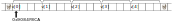
\includegraphics[scale=0.8]{img/vector.pdf}
    \end{center}
\end{frame}

\begin{frame}[fragile]{Vectores}
    Si rememoramos el ejemplo de la primera clase:\\
    \bigskip
    \begin{beamercolorbox}[wd=0.9\textwidth,sep=0.5em]{coloredboxstuffVerde}
    \verb|section .rodata:|\\
    \verb|msg: DB 'Hola mundo', 10, 0|\\
    \verb|largo: EQU $-msg-1|
    \end{beamercolorbox}
    \bigskip
    \pause
    \texttt{msg} es una etiqueta que, vista como un puntero, es un vector de caracteres almacenados de la siguiente manera:
    \begin{center}
    
\includegraphics[scale=0.6,keepaspectratio]{img/holamundo.pdf}
    \end{center}
    \pause
    \small \texttt{msg} es un \texttt{char*}, es como si en \texttt{C} hiciéramos:\\
    \small
    \begin{beamercolorbox}[wd=0.9\textwidth,sep=0.5em]{coloredboxstuffVerde}
    \verb|char msg[11] = "Hola mundo\n";|
    \end{beamercolorbox}
\end{frame}

\begin{frame}[fragile,t]{Vectores}
    Dado:\\
    \vskip 5pt
    \begin{beamercolorbox}[wd=0.9\textwidth,sep=0.5em]{coloredboxstuffVerde}
    \verb|int v[5];|\\
    \end{beamercolorbox}
    \pause
    Si suponemos que el primer elemento se encuentra almacenado\\  en la dirección 0x200 de memoria\\
    \vskip 5pt
    ¿cómo se realiza la siguiente asignación?
    \pause
    \vskip 5pt
    \begin{beamercolorbox}[wd=0.9\textwidth,sep=0.5em]{coloredboxstuffVerde}
    \verb|v[2] = 8;|
    \pause
    \end{beamercolorbox}
    \begin{textblock}{50}(10,59) \only<4->{\includegraphics[scale=0.8]{img/vectorAnimado-layer1.pdf}} \end{textblock}
    \begin{textblock}{50}(10,59) \only<5->{\includegraphics[scale=0.8]{img/vectorAnimado-layer2.pdf}} \end{textblock}
    \begin{textblock}{50}(10,59) \only<6->{\includegraphics[scale=0.8]{img/vectorAnimado-layer3.pdf}} \end{textblock}
    \begin{textblock}{50}(10,59) \only<7->{\includegraphics[scale=0.8]{img/vectorAnimado-layer4.pdf}} \end{textblock}
    \begin{textblock}{50}(10,59) \only<8->{\includegraphics[scale=0.8]{img/vectorAnimado-layer5.pdf}} \end{textblock}
\end{frame}

\begin{frame}[fragile]{Vectores} 
    En general:\\
    \vskip 3pt
    \begin{beamercolorbox}[wd=1\textwidth,sep=0.5em]{coloredboxstuffNaranja}
    \vspace{-0.55cm}
    \begin{center}
    \begin{tabular}{clclc}
    puntero al inicio & + & tamaño del dato & * & índice del elemento
    \end{tabular}
    \end{center}
    \vspace{-0.5cm}
    \end{beamercolorbox}
    \pause
    \vskip 5pt
    \begin{center}
    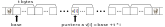
\includegraphics[scale=0.8]{img/vectorGenerico.pdf}
    \end{center}
    \vskip 5pt
    \pause
    \textit{En Intel:}\\
    \small
    \vskip 3pt
    Si el tamaño de los elementos es un valor válido como escala,
    \vskip 3pt
    \begin{beamercolorbox}[wd=1\textwidth,sep=0.5em]{coloredboxstuffNaranja}
    \verb|[ <base> + <indice> * <scale> ]| $\xrightarrow[]{\text{ejemplo}}$ \verb|[rax+rbx*4]|
    \end{beamercolorbox}
\end{frame}

\begin{frame}[fragile]{Vectores y Punteros}
    Si tenemos:
    \vskip 5pt
    \begin{beamercolorbox}[wd=1\textwidth,sep=0.5em]{coloredboxstuffVerde}
    \verb|int v[5];| 
    \end{beamercolorbox}
    \vskip 5pt
    \textit{v} es un puntero al primer elemento del vector.\\ 
    \vskip 15pt
    \pause
    Luego, vale en \texttt{C}:
    \vskip 15pt
    \begin{beamercolorbox}[wd=1\textwidth,sep=0.5em]{coloredboxstuffVerde}
    \verb| int *p_v = v;| $\leftarrow$ \footnotesize tomo el puntero al vector
    \end{beamercolorbox}
    \begin{center}
    \vskip -7pt
    ó
    \end{center}
    \begin{beamercolorbox}[wd=1\textwidth,sep=0.5em]{coloredboxstuffVerde}
    \verb| int *p_v = &v[0];| $\leftarrow$ \footnotesize tomo la dirección del primer elemento
    \end{beamercolorbox}
\end{frame}
    
\begin{frame}[fragile]{Matrices}
    \begin{itemize}
    \setlength\itemsep{0.5cm}
    \large
    \item Se representan en memoria como un \textbf{vector de vectores}.
    \pause
    \item Si la matriz tiene dimensión $M x N$ entonces sabemos que\\ está formada por $M$ vectores de $N$ elementos cada uno.
    \pause
    \item En C, las matrices se almacenan por filas.
    \end{itemize}
\end{frame}    
    
\begin{frame}[fragile]{Matrices}
    \framesubtitle{Ejemplo}
    Si tenemos \textit{M}, una matriz de enteros de $3 x 3$:
    \vskip 15pt
    \begin{center}
    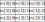
\includegraphics[scale=0.7,keepaspectratio]{img/matriz.pdf}
    \end{center}
    \vskip 15pt
    \pause
    En memoria se representa:
    \vskip 5pt
    \begin{center}
    
\includegraphics[scale=0.7,keepaspectratio]{img/matrizMemoria.pdf}
    \end{center}
\end{frame}        

\begin{frame}[fragile,t]{Matrices}
    Sí el primer elemento de \textit{M} se almacena en la dirección \texttt{0x300}.\\
    Y queremos asignar el valor \texttt{7} en $M[2,1]$ en \texttt{C}:
    \vskip 5pt
    \pause
    \begin{beamercolorbox}[wd=1\textwidth,sep=0.5em]{coloredboxstuffVerde}
    \large
    \verb|int m[3][3];|\\
    \verb|m[2][1] = 7;|
    \end{beamercolorbox}
    \pause
    \hspace{10,5cm}¿Y en ensamblador?
    \begin{textblock}{50}(30,40) \only<4->{\includegraphics[scale=0.7,keepaspectratio]{img/matrizAnimada-layer1.pdf}} \end{textblock}
    \begin{textblock}{50}(30,40) \only<5->{\includegraphics[scale=0.7,keepaspectratio]{img/matrizAnimada-layer2.pdf}} \end{textblock}
    \begin{textblock}{50}(30,40) \only<6->{\includegraphics[scale=0.7,keepaspectratio]{img/matrizAnimada-layer3.pdf}} \end{textblock}
    \begin{textblock}{50}(30,40) \only<7->{\includegraphics[scale=0.7,keepaspectratio]{img/matrizAnimada-layer4.pdf}} \end{textblock}
    \begin{textblock}{50}(30,40) \only<8->{\includegraphics[scale=0.7,keepaspectratio]{img/matrizAnimada-layer5.pdf}} \end{textblock}
    \begin{textblock}{50}(30,40) \only<9->{\includegraphics[scale=0.7,keepaspectratio]{img/matrizAnimada-layer6.pdf}} \end{textblock}
\end{frame}

\begin{frame}[fragile]{Matrices} 
    En general, para una matriz $M[i,j]$:\\
    \bigskip
    \begin{beamercolorbox}[wd=1\textwidth,sep=0.5em]{coloredboxstuffNaranja}
    \begin{center}
    \small
    \vspace{-0.5cm}
    \begin{tabular}{clclclclclc}
    puntero al inicio & + & tamaño dato & * & índice fila    & * & tamaño fila\\
                      & + & tamaño dato & * & índice columna &   & \\
    \end{tabular}
    \end{center}
    \vspace{-0.5cm}
    \end{beamercolorbox}
    \vskip 5pt
    \pause
    \textit{En Intel:}\\
%     \small
    \vskip 3pt
    Si el tamaño de los elementos es un valor válido como escala,
    \vskip 3pt
    \begin{beamercolorbox}[wd=1\textwidth,sep=0.5em]{coloredboxstuffNaranja}
    \small
    \pause
    \textcolor{black}{Primero obtengo el offset de la fila}\\
    \verb|<índiceFila> * <tamañoDato*tamañoFila>|\\
    $\xrightarrow[]{\text{ejemplo}}$ \verb|mul rax, rdx ; ojo! modifica rdx también|\\
    \vskip 5pt
    \pause
    \textcolor{black}{Segundo el offset dentro de la fila}\\
    \verb|[<índiceFila*tamañoDato*tamañoFila> + <índiceColumna> * <tamañoDato>]|\\
    $\xrightarrow[]{\text{ejemplo}}$ \verb|lea rsi, [rax+rcx*2]; rsi <= rax+rcx*2| \\
    \vskip 5pt
    \pause
    \textcolor{black}{Tercero, accedo al dato}\\
    \verb|[<base> + <índiceFila*tamañoDato*tamañoFila+índiceColumna*tamañoDato>]|\\
    $\xrightarrow[]{\text{ejemplo}}$ \verb|mov rdx, [rbx+rsi] |\\
    \end{beamercolorbox}
\end{frame}

\begin{frame}[fragile]{Matrices y Punteros}
    Si tenemos:
    \vskip 5pt
    \begin{beamercolorbox}[wd=1\textwidth,sep=0.5em]{coloredboxstuffVerde}
    \verb|int m[3][4];| 
    \end{beamercolorbox}
    \pause
    \vskip 5pt
    \textit{m} es un puntero al primer elemento de la matriz.\\ 
    \vskip 15pt
    Luego, vale en \texttt{C}:
    \vskip 15pt
    \begin{beamercolorbox}[wd=1\textwidth,sep=0.5em]{coloredboxstuffVerde}
    \verb| int *p_m = (int*)m;| $\leftarrow$ \footnotesize tomo el puntero a la matriz
    \end{beamercolorbox}
    \begin{center}
    \vskip -7pt
    ó
    \end{center}
    \begin{beamercolorbox}[wd=1\textwidth,sep=0.5em]{coloredboxstuffVerde}
    \verb| int *p_m = &m[0][0];| $\leftarrow$ \footnotesize tomo la dirección del primer dato
    \end{beamercolorbox}
\end{frame}

\begin{frame}[fragile]{Notación en C}
    Declaración y \emph{cast} de un puntero a un puntero a matriz:
    \vskip 15pt
    \begin{beamercolorbox}[wd=1\textwidth,sep=0.5em]{coloredboxstuffVerde}
    \small
    \verb|int (*matrix)[rowSize] = (int (*)[rowSize]) p;| 
    \end{beamercolorbox}
    \small
    \pause
    \vskip 15pt
    Se declara la variable \verb|matrix| como un \textbf{puntero a una matriz}.\\
    \pause
    \vskip 5pt
    \verb|p| es un \textbf{puntero a memoria} que se transforma a matriz.\\
    \pause
    \vskip 5pt
    \verb|rowSize| es la cantidad de datos en una fila (columnas)\\
    \pause
    \vskip 5pt
    Como es un puntero, no se declara la cantidad total de filas.\\
    \pause
    \vskip 20pt
    Esta sintaxis se puede utilizar para declarar matrices de N dimensiones.
    \vskip 2pt
    \begin{beamercolorbox}[wd=1\textwidth,sep=0.5em]{coloredboxstuffVerde}
    \verb|t (*m)[a]...[z] = (t (*)[a]...[z]) p;| 
    \end{beamercolorbox}
\end{frame}

\begin{frame}[fragile]{Ejercicios}
\small
    \textbf{Ejercicio 1}\\
    \verb|short suma(short* vector, short n);|\\
    Dado un vector de \textit{n} enteros de 16 bits, devolver la suma de los elementos.\\
    \vskip 5pt
    \textbf{Ejercicio 2}\\
    \verb|void diagonal(short* matriz, short n, short* vector);|\\
    Dada una matriz de \texttt{n}$\times$\texttt{n} enteros de 16 bits, devolver los elementos de la diagonal en el vector pasado por parámetro.\\
    \vskip 5pt
    \textbf{Ejercicio 3}\\
    \verb|void gris(pixel* matriz, short n, uint8_t* resultado)|\\
    Dada una matriz de \verb|n|$\times$\verb|n| pixeles RGB (1 byte por componente), hacer una función que convierta los pixeles a escala de grises usando la formula $(R+2 \cdot G+B)/4$.\\
    \vskip 5pt
    \textbf{Ejercicio 4}\\
    \verb|int* primerMaximo(int (*matriz)[sizeC], int* f, int* c);|\\
    Dada una matriz de \texttt{f}$\times$\texttt{c} enteros de 32 bits, encontrar el primer máximo buscando en el orden de la memoria. Devuelve un puntero a este valor y sus coordenadas en \texttt{f} y \texttt{c}\\
\end{frame}

% \begin{frame}[fragile]{Ejercicios}
% \textbf{Ejercicio 1 - Solución}
% \begin{columns}[t]
% \column{.48\textwidth}
% \begin{semiverbatim}
% suma:
%     ; RDI = vector
%     ; SI = n
%     
%      push rbp
%      mov rbp, rsp
%      push r12
%      
%      xor r12, r12
%      xor rcx, rcx    
%      mov cx, si
% \end{semiverbatim}
% \column{.48\textwidth}
% \begin{semiverbatim}
% .cicloSuma:
%      add r12w, [rdi]
%      lea rdi, [rdi+2] 
%      loop .cicloSuma
%      
% mov rax, r12
% 
% .fin:
%      pop r12
%      pop rbp
%      ret
% \end{semiverbatim}
% \end{columns}
% \end{frame}

% \begin{frame}[fragile]{Ejercicios}
% \textbf{Ejercicio 2 - Solución}
% \begin{columns}[t]
% \column{.48\textwidth}
% \begin{semiverbatim}
% diagonal:
%     ; rdi <-- matriz
%     ; rsi <-- filas/columnas
%     ; rdx <-- vector
% 
%     shl rsi, 48
%     shr rsi, 48
% 
%     lea r8, [rsi*2 + 2]
%     mov rcx, 0
% \end{semiverbatim}
% \column{.48\textwidth}
% \begin{semiverbatim}
%     .ciclo:
%         mov ax, [rdi]
%         mov [rdx], ax
% 
%         add rdi, r8
%         add rdx, 2
% 
%         inc rcx
%         cmp rcx, rsi
%         jne .ciclo
%     ret
% \end{semiverbatim}
% \end{columns}
% \end{frame}    

\begin{frame}[fragile]
    \frametitle{Bibliografía: Fuentes y material adicional}
    \begin{itemize}
    \item Convenciones de llamados a función en x86: \\
    \url{https://en.wikipedia.org/wiki/X86_calling_conventions}
    \item Notas sobre System V ABI: \\
    \url{https://wiki.osdev.org/System_V_ABI}
    \item Documentación de NASM: \\
    \url{https://nasm.us/doc/}
    \item Artículo sobre el flag \texttt{-pie}: \\
    \url{https://eklitzke.org/position-independent-executables}
    \item Documentación de System V ABI: \\
    \url{https://uclibc.org/docs/psABI-x86_64.pdf}
    \item Manuales de Intel: \\
    \url{https://software.intel.com/en-us/articles/intel-sdm}
    \end{itemize}
\end{frame}

\begin{frame}[plain]
    \begin{center}
    \vspace{2cm}
    \huge ¡Gracias!\\
    \vspace{2cm}
    \normalsize Recuerden leer los comentarios al final de \\ este video por aclaraciones o fe de erratas.
    \end{center}
\end{frame}

\end{document}
